\documentclass[10pt]{article}
\usepackage{enumitem}
\usepackage{hyperref}
\usepackage{float}
\usepackage{graphicx}

\title{UML modelling\\SEM-Group 86}
\author{
	Ivar de Bruin\\
	4944135
	\and
	Tim Anema\\
	4953940
	\and
	Laura Pircalaboiu\\
	4777778
	\and
	Marc Otten\\
	4872541\\
	\and
	Ilya Grishkov\\
	4770811	
}

%forces a pagebreak before a new section
\let\oldsection\section
\renewcommand\section{\clearpage\oldsection}

\begin{document}
\maketitle
\pagebreak
\tableofcontents
\section{Modelling class diagrams}
\subsection{Diagram}
		\begin{figure}[H]
			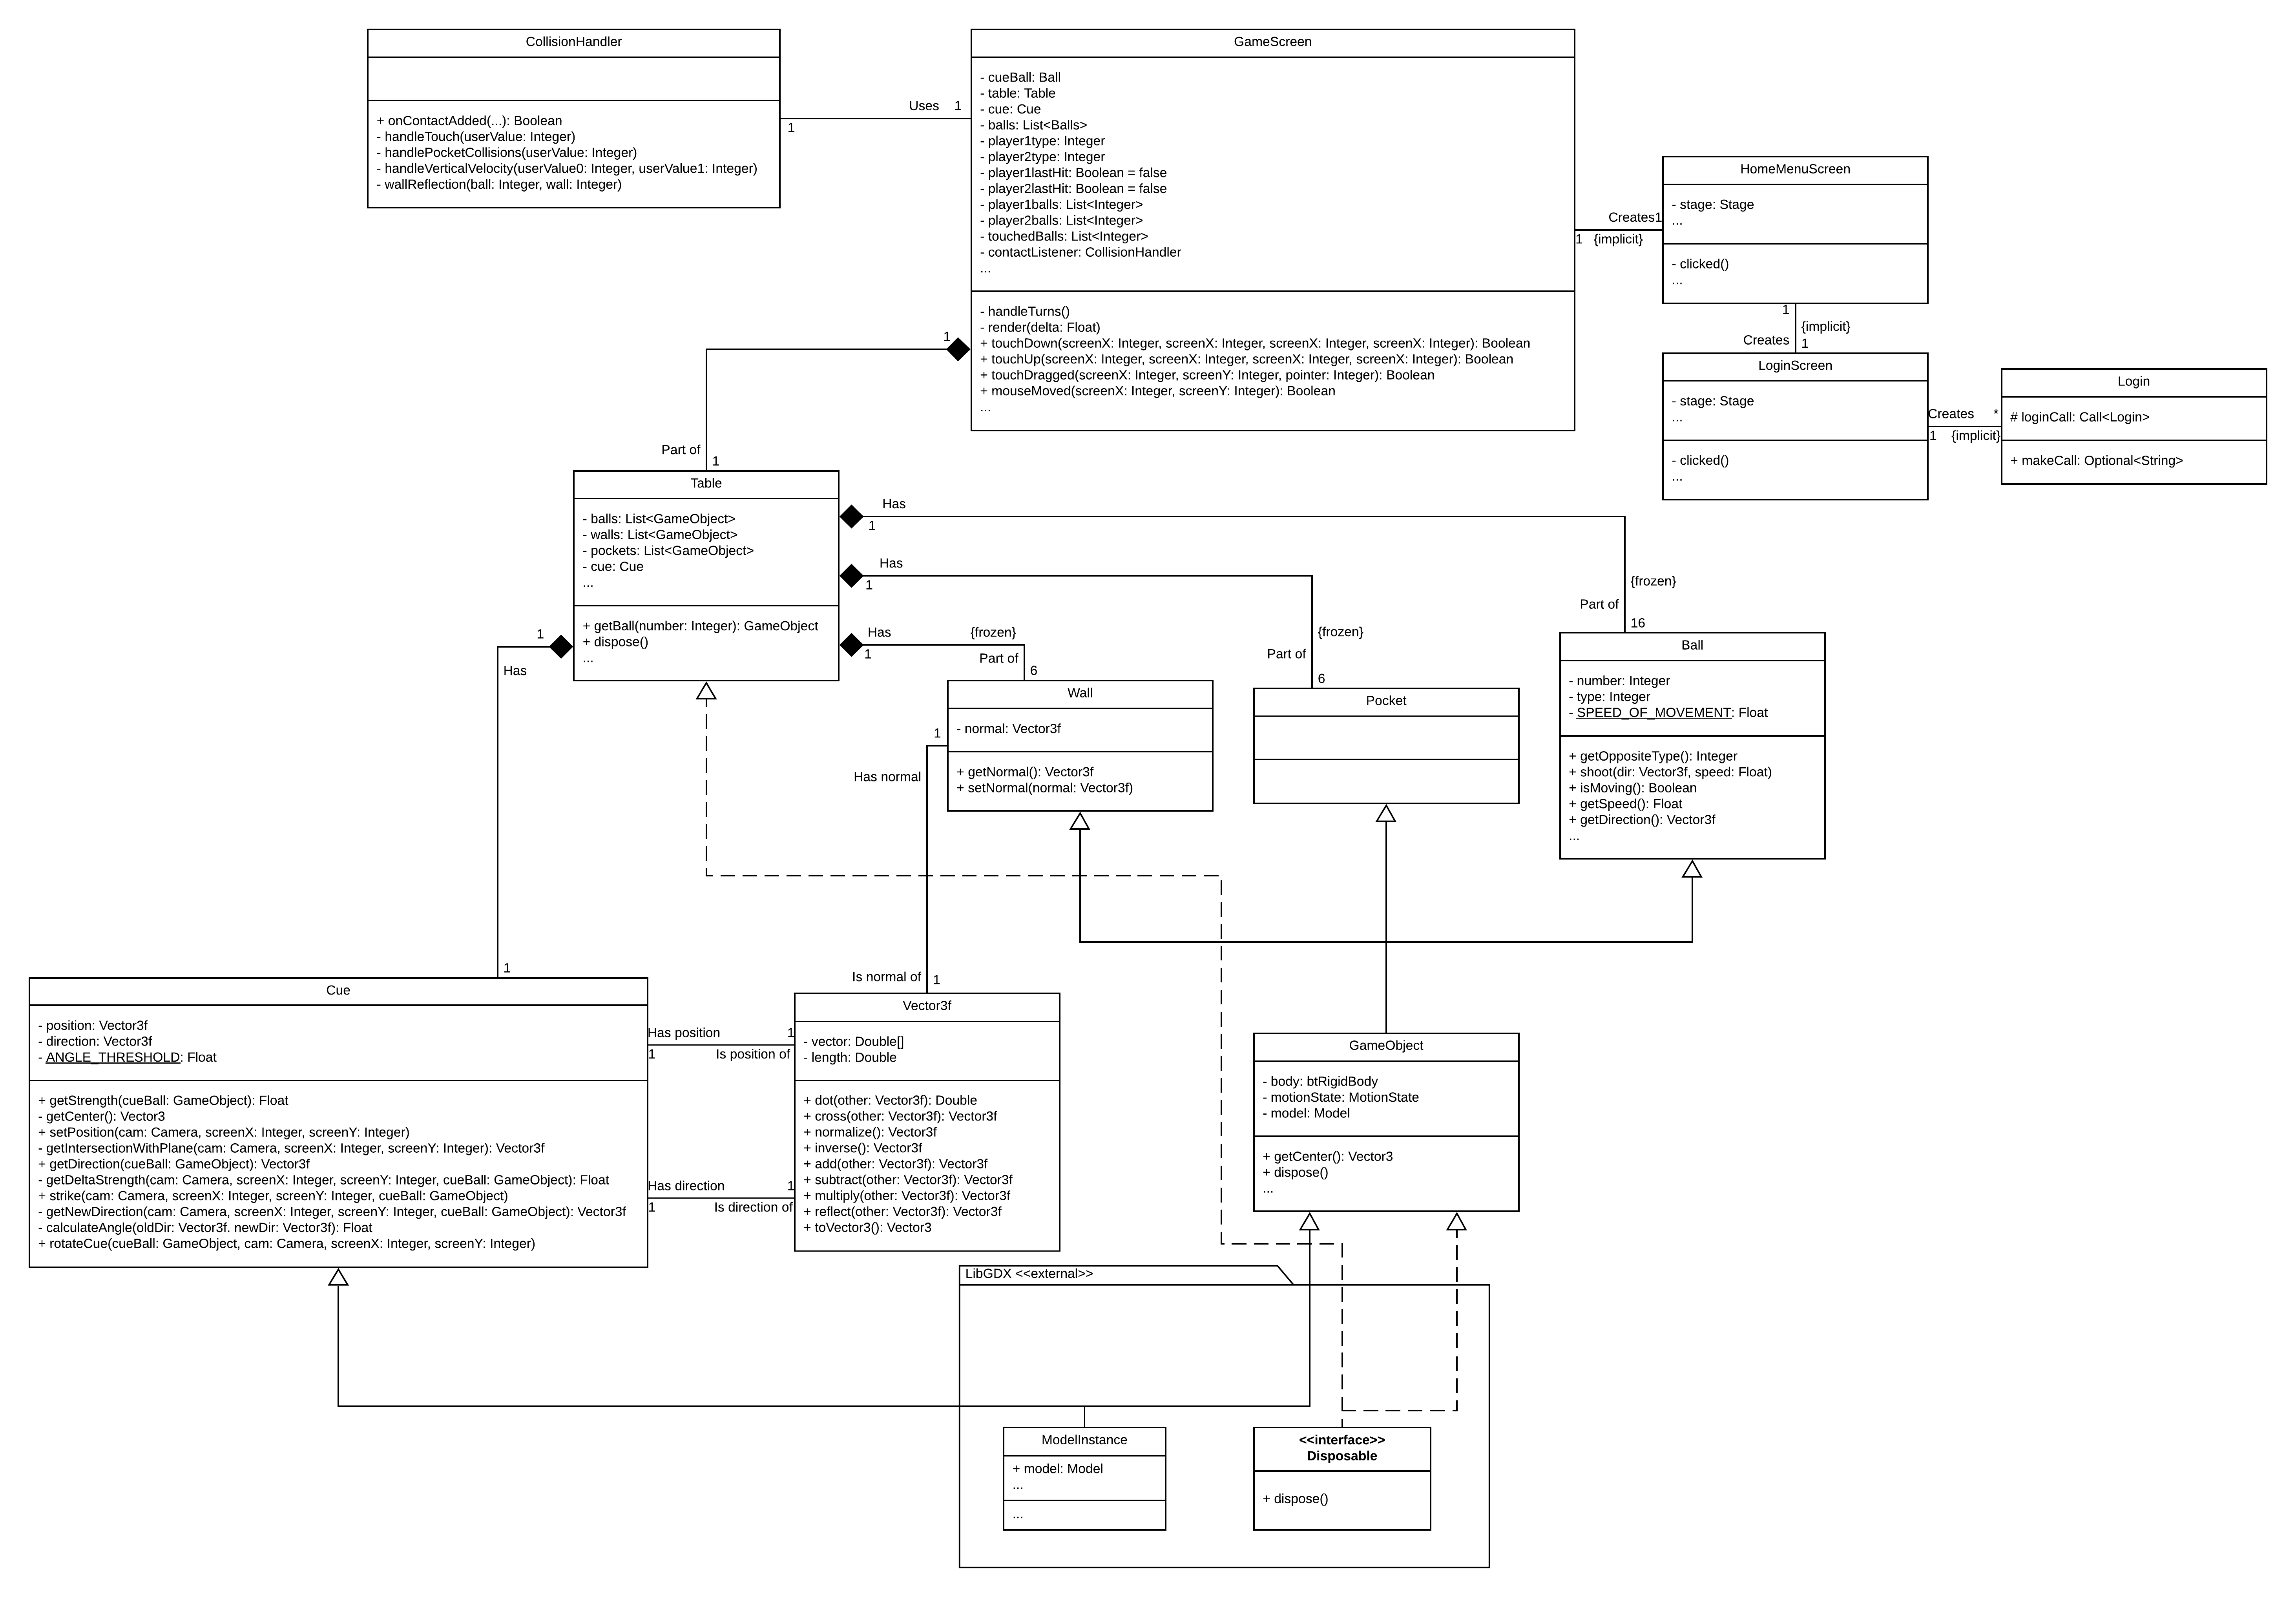
\includegraphics[width=\linewidth]{latex_images/class_diagram.png}
			\caption{Class diagram (higher res version can be found in the repository)}
		\end{figure}
		
\subsection{Explanation}
\par We choose to model GameScreen, CollisionHandler, Table, Wall, Pocket, Ball, Cue and Login. Besides those classes we also modelled classes which explain links and are important.
\par Five classes -Table, Wall, Pocket, Ball and Cue- are most certainly part of the core logic, because they represent the objects in our game and contain logic (although some more than others) which make our game tick. Besides those obvious choices we also added GameScreen, CollisionHandler and Login, because the first two contain a major part of our physics logics and the final class (Login) is what makes sure the user can actually authenticate.

\par Besides those classes we added classes which are important to understand the links between classes (take LoginScreen and HomeMenuScreen for example), classes which are superclasses of our core classes (Take GameObject and some external LibGDX classes), and classes which contain logic that is fundamental to our physics (Vector3f).


\section{Modelling Sequence diagrams}
	\subsection{Sequence diagram for authenticating a login}
		\begin{figure}[H]
			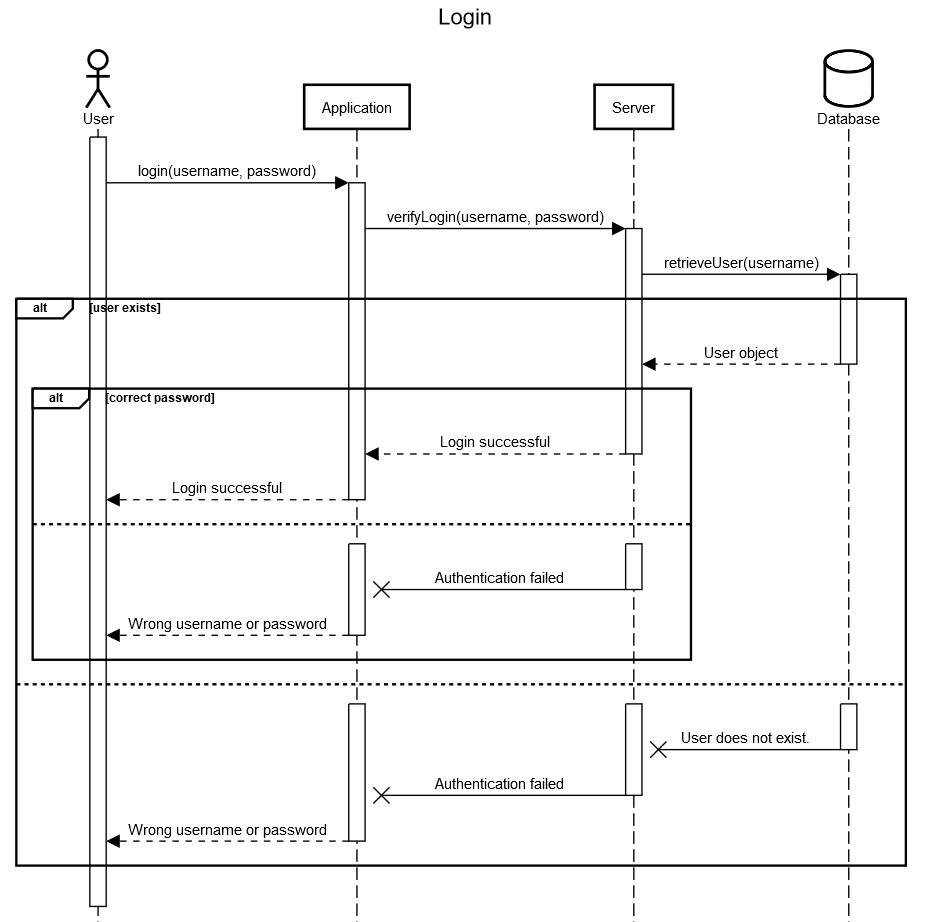
\includegraphics[width=\linewidth]{latex_images/sequenceLogin.png}
			\caption{Sequence diagram for authenticating a login(Use case 1, assignment 1)}
		\end{figure}
	\subsection{Sequence diagram for registering a new user}
		\begin{figure}[H]
			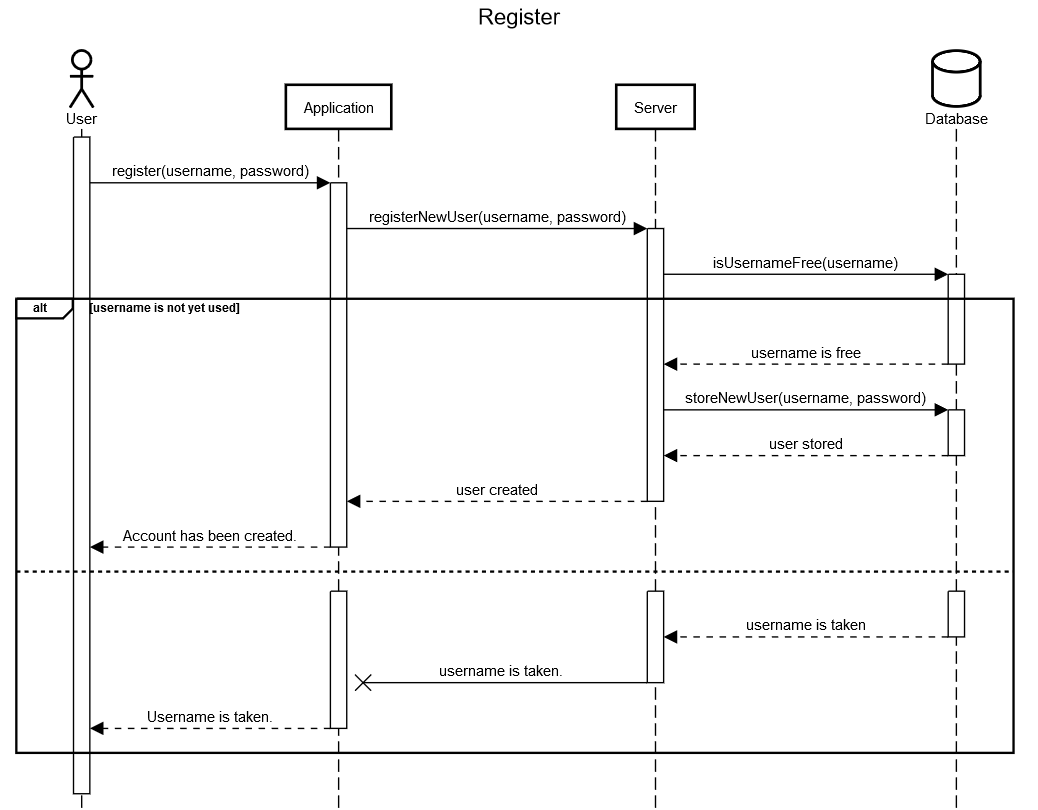
\includegraphics[width=\linewidth]{latex_images/sequenceRegister.png}
			\caption{Sequence diagram for registering a new user(Use case 2, assignment 1)}
		\end{figure}
	\subsection{Sequence diagram for adding the game score and showing the leaderboard to the user}
		\begin{figure}[H]
			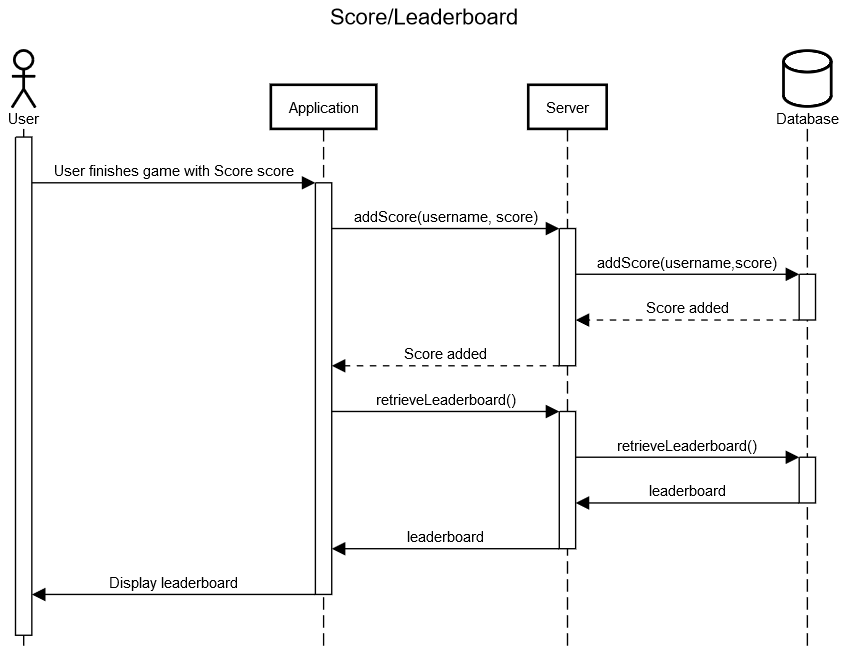
\includegraphics[width=\linewidth]{latex_images/sequenceLeaderboard.png}
			\caption{Sequence diagram for showing the leaderboard after adding the achieved score(Use case 6, assignment 1)}
		\end{figure}
\end{document}